\documentclass[12pt,a4paper,polish]{article}
\topmargin -1.6cm
\addtolength{\textheight}{4cm}
\textwidth  15.5cm

\leftmargin      5mm
\rightmargin     5mm
\oddsidemargin   5mm
\evensidemargin  5mm

\usepackage{hyperref}
\usepackage{polski}
\usepackage[utf8]{inputenc}
\usepackage{graphicx} % To jest pakiet do grafiki.
                      % Moze przydac sie pozniej.
\usepackage{units}
\usepackage{sty/wds}


\wdsTytulProjektu{RoboVision}
\wdsAutor{Marcin Bober, 249426}




\begin{document}
%
% To po to, aby mieć format A4.
% pdflatex domyślnie tworzy dokument w formacie letter.
%
\pdfpageheight   297mm
\pdfpagewidth    210mm

\wdsStronaTytulowa
\wdsSpisTresci


 \section{Charakterystyka tematu projektu}
 \label{sekcja-charakterystyka}

  Projekt ma na celu stworzenie aplikacji okienkowej, która poprzez połączenie
  internetowe będzie w stanie wydawać polecenia do robota mobilnego, sterować nim,
  a także pobierać informacje z czujników i wizualizować je.

 \section{Podcele i etapy realizacji projektu}

  Projekt powdzielony będzie na kilka pomniejszych celów tak, aby każdy z nich
  mógłbyć osobno rozwijany. \\

  Lista podelów:
  \begin{itemize}
    \item Zapoznanie się z dostępną literaturą związaną z tematem oraz zdobycie 
    informacji niezbędnych do zrealizowania zadania.
    \item Przygotowanie graficznego szkicu aplikacji wraz z rozplanowaniem funkcionalności.
    \item Zdefiniowanie protokołu komunikacyjnego, struktury ramek przesyłanych danych
     i implementacja interfejsu sieciowego.
    \item Parsowanie danych odbieraych z robota.
    \item Przygotowanie wizualizacji zebranych danych.
    \item Obsługa klawiatury i joysticka.
    \item Implementacja algorytmu sterowania i przesyłanie wyników do urządzenia.
  \end{itemize}

 \section{Specyfikacja finalnego produktu}

  Aplikacja będzie w stanie wizualizować dane odbierane z czujników robota.
  Będą to między innymi:
  \begin{itemize}
    \item wskazania akcelometru,
    \item wskazania żyroskopu,
    \item aproksymacja poziomu baterii,
    \item odlegość przeszkody zczytanej z przedniego czujnika ultradzwiękowego,
    \item prędkość rzeczywista pojazdu z enkoderów.
  \end{itemize}
  

  \newpage
  \section{Terminarz realizacji poszczególnych podcelów 
     {\small (z dokładnością do 1 tygodnia)}}

  \begin{itemize}
    \item 22 marca 2020  -- zakończenie przeglądu materiałów
                            związanych z danym tematem
    \item 29 marca 2020 -- przygotowanie schematu widoku aplikacji
    \item 12 kwietnia 2020 -- oprogramowanie obsługi joysticka
    \item 19 kwietnia 2020 -- zdefiniowanie protokołu komunikacji i budowy przesyłanych ramek
    \item 26 kwietnia 2020 -- przygotowanie logiki sterownia
    \item  4 maja 2020 -- implementacja dwustronnej komunikacji z robotem
    \item 10 maja 2020 -- wizualizacja wskazań prędkości i naładowania baterii
    \item 17 maja 2020 -- wizualizacja wskazań akcelometru
    \item 24 maja 2020 -- przygotowanie wizualizacji obiektu 3D
    \item 31 maja 2020 -- implementacja obracania obiektu 3D przy użyciu żyroskopu
    \item  7 czerwca 2020 -- szukanie błędów i testowanie wszystkich funkcji
    \item 14 czerwca 2020 -- ostateczne testy działania aplikacji
  \end{itemize}

  \begin{figure}[ht]
    \centering
    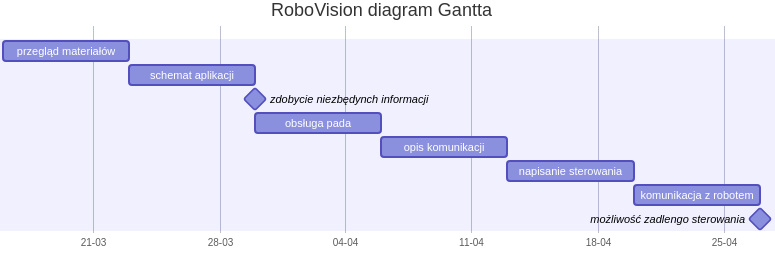
\includegraphics[width=1\textwidth]{img/gantt1.png}
    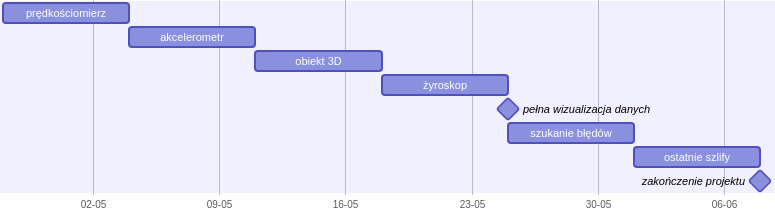
\includegraphics[width=1\textwidth]{img/gantt2.png}
    \caption{Diagram Gantta}
    \label{fig:ogniwa}
  \end{figure}


  \newpage

  \section{Projekt interfejsu graficznego}
  \begin{figure}[ht]
    \centering
    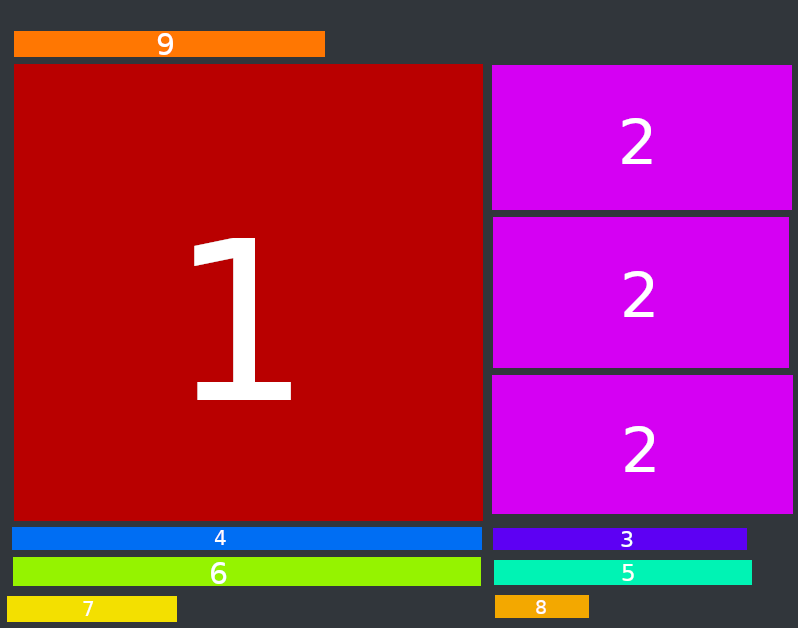
\includegraphics[width=1\textwidth]{img/schemat2.png}
    \caption{szablon interfejsu graficznego}
    \label{fig:interfejs}
  \end{figure}

  Największy wycinek okna przeznaczony jest na prezentowanie modelu
  robota w trójwymiarze (1). Obiekt ten będzie obracał się zgodnie z
  wskazaniami akcelometru zamontowanego na realnym pojeżdzie. Będzie
  więc to wizualizacja ustawienia robota w przestrzeni.

  Po prawej stonie widniejąc trzy wykresy prezentujące pomiary
  akcelometru w 3 osiach (2). Poniżej znajdują się kolejno wskażniki 
  opóźnienia  komunikacji (3), prędkości liniowej pojazdu (4) i odległości od
  przeszkody (5), a także poziom naładowania baterii (6).

  Na dolnej belce umieszczona jest informacja o podłączonym kontrolerze (7),
  i słownym statusie komunikacji z robotem (8).
  
  Na szczycie aplikacji znajduje się belka narzędziowa (9), która zawiera 
  opcję nawiązania/zerwania połączenia, wyjście z programu i informację
  o autorze aplikacji. Po wybraniu funkcji połączenia z robotem, 
  wyświetli się dodatkowe okienko z możliwością wprowadzenia adresu 
  sterowanego obiektu i przycisk umożliwiający inicjację połączenia.
  
  \section{Komunikacja z robotem}

  Połączenie z robotem odbywa się poprzez sieć WiFi. W pierwszej kolejności 
  nawiązywane jest połączenie przy użyciu protokołu TCP. Jeśli się ono powiedzie
  to uruchamiana jest dodatkowa transmicja z wykorzystaniem UDP. 
  Dzięki takiej koncepcji mamy dwa niezależne kanały komunikacji. Pierwszy służy
  do przesyłania danych które mają niski piorytet czasowy, potrzebują potwierdzenia
  odebrania i ewentualnej retransmisji danych. Druga droga komunikacji powstała, 
  aby przesyłać ciągły strumień nowych danych. Zależy nam na jaknajniższym opóźnieniu,
  a ewentualny błąd trasmisji nie jest krytyczny, bo inforamcje te szybko się 
  przedawniają i są zastępowane przez nowe, świeższe. \newline

  Każda ramka zaczyna się od wybranej dużej litery alfabetu, określającej rodzaj 
  przesyłanych danych. Dla protokołu TCP są to:

      \begin{itemize}
        \item P - ping,
        \item D - dystans przeszkody,
        \item B - bateria,
        \item S - realna predkość.
      \end{itemize}
      
  Natomiast dla protokołu UDP wyróżniamy:
    \begin{itemize}
      \item E - moc silników,
      \item A - akcelometr,
      \item G - żyroskop.
    \end{itemize}

  Wszystkie paczki danych zakończone są średnikiem, przed którym znajduje się
  ośmiobitowy cykliczny kod nadmiarowy. Niestety ze względu na róźnorodność 
  transmitownych informacji, w tym miejscu kończą się cechy wspólne poszczególnych 
  ramek.

  \subsection{Ping}
  Jest to najprostrza z obecych tu ramek. Nie przenosi żadnych informacji.
  Oznacza jedynie koniecność odesłania do nadawcy identyczniej wiadomości,
  aby można było wyznaczyć chwilę czasowe, niezbędne do obliczenia opóźnienia
  transmisji.

  Forma ramki to: $P\#;$

  Gdzie \# oznacza CRC.



  \subsection{Dystans przeszkody}
  Przesyła informacje z robota o odległości odczytanej z czujnika ultradzwiękowego.
  
  Forma ramki to: $D<uint8\_t>\#$;
  \newline

  Gdzie \# oznacza CRC. Przed nim znajduje się wartość odległości wyrażonej 
  w centymetrach, w zakresie 0-100cm.



  \subsection{Bateria}
  Przesyła informacje z robota o poziomie baterii.

  Forma ramki to: $B<uint8\_t>\#$;
  \newline

  Gdzie \# oznacza CRC. Przed nim znajduje się poziom baterii wyrażonej 
  w procentach, w zakresie 0-100\%.



  \subsection{Prędkość}
  Przesyła informacje z robota o prędkości na kołach.

  Forma ramki to: $S<uint8\_t> <uint8\_t>\#$;
  \newline

  Gdzie \# oznacza CRC. Przed nim znajdujdują się dwie wartości oddzielone spacją
  odnoszące się do prędkości poszczególnych kół wyrażonej w metrach na sekunde.



  \subsection{Moc silników}
  Przesyła informacje z aplikacji do robota o zadanej mocy silników.

  Forma ramki to: $E<uint8\_t> <uint8\_t>\#$;
  \newline

  Gdzie \# oznacza CRC. Przed nim znajdujdują się dwie wartości oddzielone spacją
  odnoszące się do zadanej mocy poszczególnych kół wyrażonej w procentach.
  Zakresy tych wartości musza mieścić się od 0 do 100\%



  \subsection{Akcelometr}
  Przesyła informacje z robota o aktualnych wskazaniach akcelometru.

  Forma ramki to: $A<uint8\_t> <uint8\_t> <uint8\_t>\#$;
  \newline

  Gdzie \# oznacza CRC. Przed nim znajdujdują się trzy wartości oddzielone spacją
  odnoszące się do aktualnych wskazań akcelometru.


  \subsection{Żyroskop}
  Przesyła informacje z robota o aktualnych wskazaniach żyroskopu.

  Forma ramki to: $G<uint8\_t> <uint8\_t> <uint8\_t>\#$;
  \newline

  Gdzie \# oznacza CRC. Przed nim znajdujdują się trzy wartości oddzielone spacją
  odnoszące się do aktualnych wskazań żyroskopu.


  \section{Aktualne rezultaty}
  Na dzień dzisiejszy, projekt nie jest obarczony żadnymi opóźnieniami. Wszystkie 
  zaplanowane kamienie milowe zostały osiągnięte przed terminem. Aplikacja może 
  poszczycić się już działającą obsługa joysticka, gotową komunikacją z robotem,
  algorytmem różnicowego układu sterowania oraz działającym wskaźnikiem opóźnienia,
  prędkości liniowej i poziomu baterii. Pozostało więc zaimplementować wizualizację
  obiektu 3D oraz wykresy przeciążeń. Ostatnia faza projektu zakłada również eliminację
  błędów.

  
\bibliographystyle{plplain}
\bibliography{baza_bibliografii}
\end{document}

